\chapter{Propuesta}\label{chapter:proposal}
En este capítulo se realiza una propuesta para atacar el problema de desarrollar un sintetizador de voz con voces cubanas. En la sección \ref{db} se comenta sobre la base de datos a contruir para el entrenamiento de modelos. Luego en las secciones \ref{taco},\ref{vits-sandra}, \ref{it-en}, \ref{angelina} se exponen los diferentes criteros a desarrollar.\\

Con el objetivo de lograr una síntesis de voz satisfactoria y después de realizar un estudio de las tecnologías que se utilizan para este fin, se elige Coqui TTS como plataforma para el entrenamiento de los nuevos modelos DNN. Coqui cuenta con una gran variedad de modelos preentrenados en más de 20 idiomas.  
El primer paso en el desarrollo del sintetizador es instalar la biblioteca Coqui TTS, de acuerdo a las indicaciones del repositorio oficial[\cite{coqui-doc}].

 Se realizó un estudio del comportamiento de parejas modelo TTS - VoCoder, para evaluar cuáles pares ofrecían mejores resultados. Es decir se tomó un modelo de la primera etapa en un sistema de dos etapas, como Tacotron2 que convierte texto en espectograma de mel, y se empareja con un VoCoder como HiFiGan para a partir del espectograma obtener una salida de audio. Las combinaciones se pueden observar en la figuras \ref{en_tacotron2}, \ref{en_fastpitch}, \ref{en_glowtts}.

Se experimenta la combinación del modelo TTS Tacotron2-DDC preentrenado en Inglés con los VoCoders WaveGrad y HiFiGan-V2 como se evidencia en la figura \ref{en_tacotron2}. Igualmente con el modelo Fast-Pitch preentrenado en inglés con el VoCoder UnivNet igualmente en inglés(figura \ref{en_fastpitch}), para terminar con los modelos en inglés se combina Glow-TTS y el VoCoder Multiband-MelGan(figura \ref{en_glowtts}).
Los modelos preentrenados en idioma inglés al combinarse con estos VoCoders, para un texto en español arrojan distintos resultados, en algunos casos solo producen señales ruidosas mientras que los más satisfactorios, producen un discurso con una pronunciación propia de una persona de habla inglesa hablando español.

\begin{figure}[H]
	\centering
	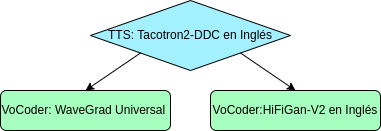
\includegraphics[width=0.6\linewidth]{Graphics/en_tacotron2}
	\caption{Modelo TTS Tacotron2-DDC entrenado en Inglés}
	\label{en_tacotron2}
\end{figure}

\begin{figure}[H]
	\centering
	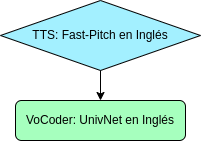
\includegraphics[width=0.3\linewidth]{Graphics/en_fastpitch}
	\caption{Modelo TTS Fast-Pitch entrenado en Inglés}
	\label{en_fastpitch}
\end{figure}
\begin{figure}[H]
	\centering
	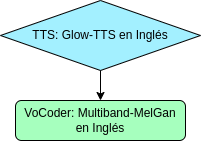
\includegraphics[width=0.3\linewidth]{Graphics/en_glowtts}
	\caption{Modelo TTS Glow-TTS entrenado en Inglés}
	\label{en_glowtts}
\end{figure}


Por otro, lado Coqui solo cuenta con un modelo preentrenado en español, el \textbf{Tacontron-DDC}, que está entrenado sobre la base de datos de M-AILABS[\cite{mailabs}]; este modelo fue probado junto a VoCoders preentrenados como se muestra en la figura \ref{es_tacotron}. Los mejores resultados fueron arrojados por las combinaciones de \textbf{Tacontron-DDC} con los modelos: Univnet entrenado sobre la base de datos LJSpeech[\cite{ljspeech}] en inglés, y Wavegrad entrenado sobre el conjunto de datos LibriTTS[\cite{libritts}][\cite{libritts1}], aunque ambos presentan problemáticas como la mala pronunciación de la letra ñ.

\begin{figure}[H]
	\centering
	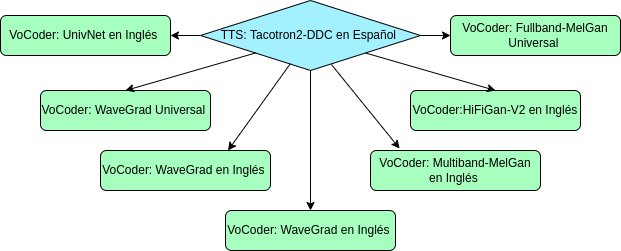
\includegraphics[width=0.8\linewidth]{Graphics/es_tacotron}
	\caption{Modelo TTS Tacotron2-DDC entrenado en Español}
	\label{es_tacotron}
\end{figure}


De acuerdo con la documentación de Coqui, el objetivo de la investigación que consiste en desarrollar un sintetizador de voz en español con voz cubana, y experimentos iniciales realizados se proponen cuatro enfoques:

\begin{enumerate}
	\item Realizar un \textit{fine-tuning} o reentrenamiento, utilizando una base de datos con voces cubanas, al modelo preentrenado de Coqui[\cite{coqui-doc}], \textbf{Tacontron-DDC}, que es el único disponible en español. 
	
	\item Realizar el entrenamiendo desde cero de un modelo, en este caso se podría entrenar cualquier modelo disponible. \textbf{VITS} es un buen candidato pues en general produce resultados bastante satisfactorios.
	
	\item Realizar un \textit{fine-tuning} a modelos \textbf{VITS} preentrenados en idiomas distintos al español.
	
	\item Realizar un preentrenamiento desde cero al modelo \textbf{VITS} utilizando una base de datos fuente en español, para luego realizar un proceso de \textit{fine-tuning} sobre este, pero utilizando la base de datos contruida con voces cubanas.
	
	
	
\end{enumerate}

Y a partir de estos evaluar y comparar resultados.

Para el desarrollo de cualquiera de los anteriores es imprescindible la construcción de un conjunto de datos que se adapten al modelo y a las necesidades de la investigación.


\section{Creación de la base de datos} \label{db}

Para entrenar un modelo TTS, se necesita un conjunto de datos con grabaciones de voz y transcripciones, en este caso fue una base de datos en español con voces cubanas. El discurso debe dividirse en clips de audio y cada clip necesita su transcripción correspondiente. La base de datos debe poseer una organización específica, de forma tal que el cargador de datos de Coqui TTS sea capaz de cargarlos para utilizar en el entrenamiento[\cite{formatting-dataset}].    

\subsubsection{Formato wav}
Los clips de audio del conjunto de datos deben poseer formato WAV. El formato WAV[\cite{wav}], es un formato estándar de archivo de audio, desarrollado por IBM[\cite{ibm}] y Microsoft[\cite{microsoft}], para almacenar un flujo de bits de audio en PC. Los archivos WAV no se comprimen cuando se codifican. Eso significa que todos los elementos del audio originales permanecen en el archivo. Los editores de audio describen los archivos WAV como ``sin pérdidas'' porque no se pierde ninguna parte de su sonido. Como resultado, los archivos WAV tienen objetivamente una mejor calidad y proporcionan clips de audio más reales y precisos. .


\subsubsection{Idioma Español}
La base de datos que se conforma debe tener una buena cobertura del idioma en el que se desea entrenar el modelo. Debe cubrir la variedad fonética, los sonidos excepcionales y los signos especiales.

El idioma español[\cite{ecured}] o castellano. Es una lengua romance del grupo ibérico, y tras el chino mandarín, es la lengua más hablada del mundo por el número de personas que la tienen como lengua materna. El idioma es un rasgo esencial de la nacionalidad. Por eso unos de los rasgos que define a los cubanos, es precisamente este: la comunicación mediante el idioma español. 

Las variedades geográficas del español, llamadas dialectos o geolectos, difieren entre sí por multitud de razones. Entre las de tipo fonético destacan la distinción o no de los fonemas correspondientes a las grafías c/z y s (ausencia o presencia de ceceo/seseo), la distinción o no de los fonemas correspondientes a las grafías ll e y (ausencia o presencia de yeísmo) y la aspiración o no de la s ó z ante una consonante, aunque estas diferencias no suelen ocasionar problemas de inteligibilidad entre sus hablantes.

La estructura silábica más frecuente del español es consonante más vocal, de forma que tiende hacia la sílaba abierta. Caracteriza al español una tensión articulatoria alta, no tan relajada como en italiano, y estadísticamente una gran presencia de la vocal a. La acentuación es de intensidad y estadísticamente dominan las palabras llanas, o acentuadas en la penúltima sílaba, después las agudas y por último las esdrújulas. 

En español hay cinco vocales fonológicas: /a/, /e/, /i/, /o/ y /u/. La /e/ y /o/ son vocales medias, ni cerradas ni abiertas, pero pueden tender a cerrarse y abrirse. Sin embargo, estos sonidos no suponen un rasgo distintivo en español general. Según la mayoría de los autores, se distinguen por lo general 24 fonemas en el español, cinco de los cuales corresponden a vocales y 19 a consonantes, además de otros fonemas dialectales y/o alofónicos\footnote{alófono: Sonido propio de la pronunciación de un fonema, que puede variar según su posición en la palabra o en la sílaba y en relación con los sonidos vecinos, aunque sigue considerándose el mismo fonema.}, aunque la mayoría de los dialectos sólo cuentan con 17 consonantes, y algunos otros con 18.

El español se escribe mediante una variante del alfabeto latino con la letra adicional ``ñ'' y los dígrafos\footnote{dígrafo: Signo ortográfico compuesto de dos letras y que representa un solo sonido.} ``ch'' y ``ll'', consideradas letras del abecedario desde 1803, debido a que representan un solo sonido, distinto de las letras que lo componen. Así, el alfabeto español queda formado por 27 letras y 2 dígrafos: a, b, c, ch, d, e, f, g, h, i, j, k, l, ll , m, n, ñ, o, p, q, r, s, t, u, v, w, x, y, z. Además el español emplea signos gráficos de interrogación y exclamación como ``¿'' y ``¡'', que no poseen otras lenguas. Estos signos especiales facilitan la lectura de interrogaciones y exclamaciones largas que oralmente solo se expresan por variaciones de entonación. 

Todos estos aspectos deben tenerse en cuenta para la conformación de una base de datos en español.

\subsubsection{¿Qué hace a una buena base de datos?}

\begin{itemize}
	\item Debe cubrir una cantidad considerable de clips cortos y largos.
	\item Libre de errores. Se debe eliminar cualquier archivo incorrecto o corrupto. 
	\item Para escuchar una voz con la mayor naturalidad posible, usar las diferencias de frecuencia y tono, y signos de puntuación.
	\item Es necesario que el conjunto cubra una buena parte de fonemas, difonemas y, en algunos idiomas, trifonemas. Si la cobertura de fonemas es baja, el modelo puede tener dificultades para pronunciar nuevas palabras difíciles.
	\item Las muestras de la base de datos deben estar lo más limpio posible, es decir, se debe limpiar de ruido y cortar los espacios de tiempo entre expresiones, donde no se hable.
	
\end{itemize}

\subsubsection{Cuban Voice Dataset}
Como resultado de la investigación es obtenida una base de voces recopilada por el autor de esta tesis, de un hablante cubano. Las grabaciones de audio se recolectaron usando la grabadora de voz de un dispositivo celular. Las sentencias grabadas consisten el fragmentos de tres libros diferentes, ``El Lobo Estepario'',  ``El Principito'', y  ``El Alquimista'', así como otras frases populares, números, y fechas.\\ 

La base de datos está conformada por 160 clips de audio con sus respectivas transcripciones recogidas en el archivo metadata.csv. Cada clip tiene una duración de 2 a 15 segundos.\\

Los clips de audio poseen formato .wav y se organizan dentro de una carpeta de nombre wavs de la siguiente forma:

\begin{center}
	/wavs\\
	| - audio1.wav\\
	| - audio1.wav\\
	| - audio2.wav\\
	| - audio3.wav\\
	...
\end{center}

Las transcripciones se recogen dentro del archivo metadata.csv. Donde audio1, audio2, etc se refieren a los archivos audio1.wav, audio2.wav etc.

\begin{center}
	audio1|Esta es mi transcripción 1.
	
	audio2|Esta es mi transcripción 2.
	
	audio3|Esta es mi transcripción 3.
	
	audio4|Esta es mi transcripción 4.
\end{center}

Se adoptará en la conformación de la base de datos con voces cubanas, la misma estructura de la base de datos en Español de \textit{The M-AiLabs Speech Dataset}, pues algunos de los modelos que se utilizaron fueron preentrenados sobre estos conjuntos de datos. Finalmente queda la siguiente organización:

\begin{flushleft}
	/[Nombre del conjunto]/by$\_$book/female/[creador]/[nombre del hablante]
	
	|/wavs
	
	|metadata.csv
\end{flushleft}

\subsection*{Fine-Tuning}
Entrenar correctamente un modelo de aprendizaje profundo requiere generalmente de una gran base de datos y de un extenso entrenamiento.

Si se dispone del material necesario y del tiempo para entrenar el algoritmo, estos requisitos no suponen ningún problema, pero, si la base de datos es pequeña o el modelo no se entrena lo suficiente, el aprendizaje podría no ser completo.

El \textit{fine-tuning} consiste en aprovechar la información que se ha aprendido de la resolución de un problema y utilizarla sobre otro distinto, pero que comparte ciertas características. Se usan los conocimientos adquiridos por una red convolucional para transmitirlos a una nueva red convolucional. Esta nueva red convolucional que se crea no tiene por qué modificar la red original y puede simplemente aprender de ella, sin embargo también es válido el caso donde no solo se modifica la red original, sino que se vuelve a entrenar para aprender más conceptos.

En la presente investigación, se utiliza el reentrenamiento, para a partir modelo previamente entrenado y realizar un nuevo entrenamiento para mejorar su rendimiento en un conjunto de datos diferente.\\

\section{Fine-Tuning de Tacontron-DDC} \label{taco}

Se implementa como primera variante el reentrenamiento(\textit{fine-tuning} en inglés) del modelo \textbf{Tacontron-DDC} en español, pues brinda ventajas tales como un aprendizaje más rápido, ya que un modelo preentrenado ya tiene aprendidas funcionalidades que son relevantes para la tarea de producir un discurso. Además convergerá más rápido en el nuevo conjunto, lo que reducirá el costo de entrenamiento y permitirá el proceso de experimentación más rápidamente. Y de acuerdo a la teoría se pueden obtener buenos resultados con un conjunto de datos más pequeño.\\

Luego de tener entrenado el modelo acústico(TTS) con una base de datos construida con voces cubanas, es posible que alguno de los VoCoders preentrenados disponibles produzca una salida con las características deseadas, en caso contrario se debería entrenar el VoCoder con los datos de la base de datos resultado de la investigación.


El proceso de \textit{fine-tuning} consiste en modificar la configuración original del modelo preentrenado seleccionado, es decir, especificar la base de datos a utilizar en el reentrenamiento, los detalles acústicos que reflejen las características del nuevo conjunto de datos, el nombre del nuevo modelo ajustado, la dirección donde se guardará el modelo reentrenado, entre otros aspectos. Para la mayoría de los parámetros se tomaron las características del modelo original \textbf{Tacontron-DDC} en español.


\section{Entrenamiento de modelo VITS desde cero} \label{vits-sandra}

Existen varios modelos de texto a voz de extremo a extremo que permiten el entrenamiento en una sola etapa y el muestreo en paralelo, sin embargo, generalmente la calidad de la muestra no coincide con la de los sistemas TTS de dos etapas. 

Se selecciona VITS porque es un método TTS paralelo de extremo a extremo que genera un sonido de audio más natural que los modelos actuales de dos etapas. Y de acuerdo a una evaluación humana subjetiva[\cite{mos}] (puntuación de opinión media, o MOS), muestra que el modelo supera a los mejores sistemas TTS disponibles públicamente y logra un MOS comparable a la realidad.

Con este enfoque se debe entrenar la DNN de VITS partiendo de cero. Una desventaja es que cae una gran responsabilidad sobre el conjunto de datos de entrenamiento, pues debe tener una gran riqueza del idioma y muchos clips de audio.
	
	
\section{Fine-tuning de modelos VITS preentrenados en otros idiomas} \label{it-en}

Se persigue experimentar el proceso de \textit{fine-tuning} en este modelo de extremo a extremo, sin embargo no existen modelos VITS preentrenados en español disponibles. Por esto se escogen los idiomas italiano e inglés como candidatos en esta tarea.

\subsection{Italiano} 
Las culturas hispánicas tienen mucho en común con la cultura italiana, sobre todo en lo que concierne al lenguaje y la comunicación. Tanto el español como el italiano son lenguas romances, derivadas del latín, siendo justamente de las más similares, incluso más que el francés o el rumano.

Es por este hecho que el italiano y el español comparten palabras muy parecidas y siguen la misma estructura gramatical. Entre ellos existe un grado de similitud léxica del 82$\%$, lo que además indica que son idiomas fáciles de aprender para sus respectivos hablantes. Sin embargo, las características que tienen en común van más allá de su origen y de la gramática.

Una similitud entre ambas lenguas es la cantidad de vocales en el alfabeto, aunque en italiano las vocales tienden a matizarse con sonidos más abiertos y con un acento grave. Es muy común que el parecido existente entre las palabras en italiano y español se vea afectada sólo por una o más vocales, como por ejemplo: vecino y vicino, cámara y camera, igual y uguale. Por supuesto existen un gran número de diferencias, aunque son más notables en vocabulario que en lo que respecta a la pronunciación. 

Debido a todo esto un modelo entrenado en italiano sería el candidato ideal para realizar un ajuste sobre una base de datos en español. 
\subsection{Inglés}

A pesar de las diferencias evidentes, en realidad el español y el inglés se parecen más de lo se cree. La primera de las semejanzas entre el inglés y el español es que usan el alfabeto romano, lo cual provoca que los sonidos de ambos idiomas sean similares, aunque no plenamente iguales. El mejor ejemplo lo constituyen las vocales: mientras en el español sólo se reconocen 5 sonidos, uno para cada vocal, en el inglés encontramos más de 14 sonidos, pues hay vocales cortas y largas, las cuales se catalogan así por la duración de su pronunciación. Estos dos idiomas son alfabéticos, de modo que a través de letras se pueden representar sus sonidos; el español comparte 2/3 de sus fonemas con el inglés.

La estructura gramatical del inglés es similar a la del español en más de un 90$\%$, pero la del inglés es muchísimo más simple. Además, el vocabulario se forma con prefijos y sufijos tanto en inglés como en español (que son en su mayoría de raíz latina en ambos idiomas).

Las consonantes v, ll, h, j, r, rr, z, y  la x son pronunciadas muy diferentes en español y en inglés. La consonante ñ no existe en inglés; el sonido que se conoce de esta consonante en español se escribe en ingles ny. Las combinaciones de algunas consonantes con vocales cambia totalmente el sentido de la pronunciación. Por ejemplo: la combinación de la “q” y la “u” en las palabras como queen, quiet o quick la pronunciación de  la “u” en inglés se percibe.

Teniendo en cuenta la similitud, y al mismo tiempo las marcadas diferencias entre ambos idiomas, se escoge un modelo VITS preentrenado en inglés para realizar un \textit{fine-tuning} con la base de datos cubana.


\section{Entrenamiento del modelo VITS con una base de datos fuente} \label{angelina}

Hasta este punto se había depositado demasiada confianza en la base de datos conformada para la investigación. Es necesario comprobar si el modelo VITS arroja buenos resultados para el idioma español, por esto se decide realizar un entrenamiento desde cero con una base de datos en español que pertenece al grupo \textit{The M-AILABS DATASET} con un hablante mexicano. Luego de esto se procede a realizar \textit{fine-tuning}, esta vez con la base de datos de voces cubanas. 

Este enfoque es el más prometedor, pues se confía en la calidad y riqueza de la base de datos fuente, para que el modelo aprende la mayoría de las peculiaridades del lenguaje, y luego en la segunda etapa solo sea una cuestión de ajuste al tono de voz del nuevo hablante cubano.